\chapter{Verwendete Tools und Hilfsfunktionen}
\label{ch:Tools}

Zur erfolgreichen Umsetzung der verschiedenen Challenges im Rahmen des Projekts kamen zwei eigenständig entwickelte Tools zum Einsatz, die gezielt zur Kalibrierung, Analyse und Datenerhebung dienten. Beide Nodes erleichterten die Entwicklung und Optimierung der Bildverarbeitung erheblich und ermöglichten eine praxisnahe Justierung des Systems.

\section{HSV-Kalibrierung}

Unterschiedliche Lichtverhältnisse, etwa durch Sonnenlicht, Schatten oder künstliche Beleuchtung, führten im Testumfeld regelmäßig dazu, dass die Fahrbahnmarkierungen nicht zuverlässig erkannt wurden. Um unter allen Bedingungen eine stabile Bildverarbeitung sicherzustellen, war daher vor jedem Arbeitstag eine Kalibrierung der Farbwerte erforderlich. Die hier eingesetzte Kalibrierungs-Node erleichterte diesen Vorgang erheblich und machte die Justierung der HSV-Werte effizient und wiederholbar.

Die \texttt{white\_yellow\_red\_calibration\_node} stellte eine interaktive Kalibrierungsumgebung bereit, in der für jede der drei Farbklassen \texttt{white}, \texttt{gelb} und \texttt{red} die sechs relevanten Parameter (Hue, Saturation, Value – jeweils untere und obere Grenze) per OpenCV-Trackbars in Echtzeit angepasst werden konnten. Die betroffenen Bildbereiche wurden live eingefärbt dargestellt, sodass sich die Wirkung der Einstellungen unmittelbar überprüfen ließ. Ein Modus-Switch ermöglichte das gezielte Umschalten zwischen den Farbklassen. Per Tastendruck konnten die jeweils eingestellten Werte gespeichert und automatisch in einer YAML-Konfigurationsdatei abgelegt werden, um sie zur Laufzeit direkt wiederzuverwenden.

Die Kalibrierung der roten Stopplinien war dabei besonders sensibel, da eine zuverlässige Trennung von Hintergrundartefakten erforderlich war. Insgesamt erwies sich die \texttt{white\_yellow\_red\_calibration\_node} als essenzielles Werkzeug, um das System auf wechselnde Lichtbedingungen vorzubereiten und eine stabile Bildverarbeitung während der Entwicklung sicherzustellen.

\begin{figure}[H]
    \centering
    \begin{subfigure}[t]{0.32\textwidth}
        \centering
        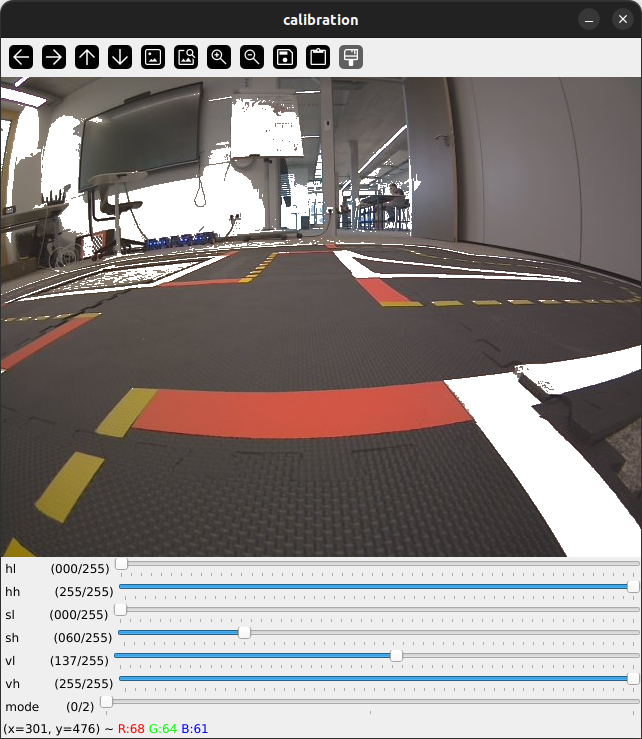
\includegraphics[width=\linewidth]{Figures/png/Kalibrierung_weiß.png}
        \caption{Weiß bei hoher Helligkeit}
        \label{fig:hsv_white}
    \end{subfigure}
    \hfill
    \begin{subfigure}[t]{0.32\textwidth}
        \centering
        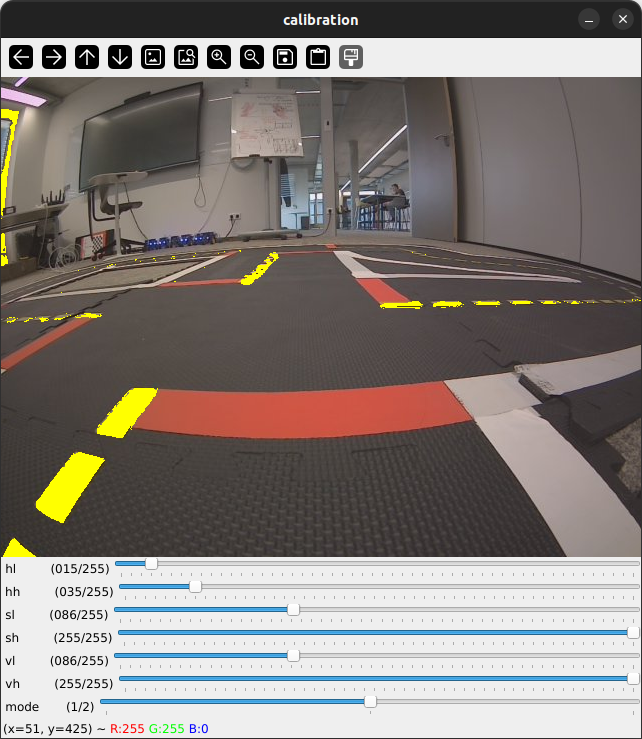
\includegraphics[width=\linewidth]{Figures/png/Kalibrierung_gelb.png}
        \caption{Gelb mit optimierter Segmentierung}
        \label{fig:hsv_yellow}
    \end{subfigure}
    \hfill
    \begin{subfigure}[t]{0.32\textwidth}
        \centering
        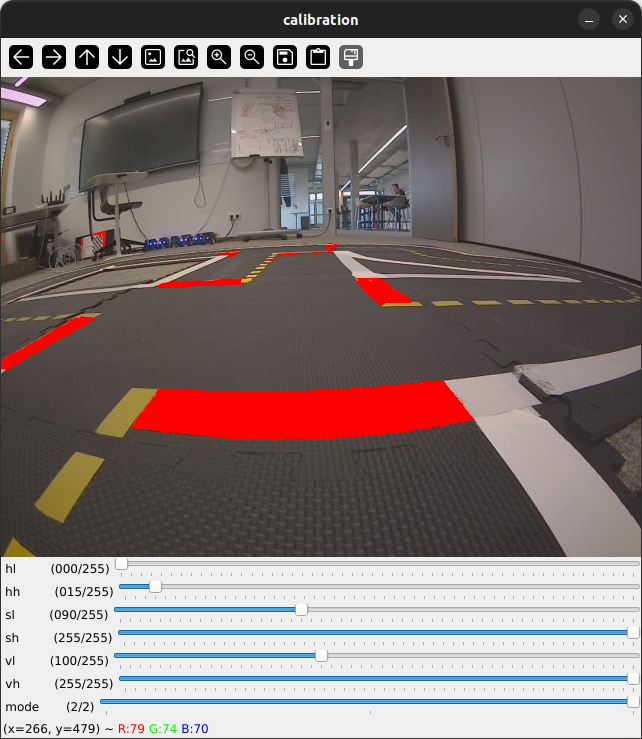
\includegraphics[width=\linewidth]{Figures/png/Kalibrierung_rot.png}
        \caption{Rot mit zweigeteilter HSV-Maske}
        \label{fig:hsv_red}
    \end{subfigure}
    \caption{Beispielhafte Kalibrierung der Farbklassen Weiß, Gelb und Rot}
    \label{fig:hsv_calibration}
\end{figure}



\section{Visuelle Kontrolle und Datensatzgenerierung}

Für die Entwicklung der Objekterkennung mit YOLO wurden umfangreiche Datensätze mit annotierten Bildern benötigt. Die \texttt{display\_and\_save\_cameraImg\_node} erfüllte in diesem Zusammenhang zwei Funktionen:
\begin{enumerate}
    \item Einerseits diente sie zur visuellen Kontrolle des Kamerabildes zur Laufzeit, 
    \item andererseits speicherte sie regelmäßig aktuelle Bildframes ab, um damit die Trainingsdatenbasis zu erweitern.
\end{enumerate}

Die Node subscribed auf das aktuelle Kamerabild des Duckiebots (komprimiertes JPEG über \ac{ROS}) und zeigt dieses in einem separaten OpenCV-Fenster an. Parallel wird in einem zyklischen Intervall von standardmäßig 3 Sekunden ein Bild aus dem Videostream unter dem angegebenen Dateipfad und -namen auf den Duckiebot abgelegt.

In einem Terminal Fenster kann daraufhin mittels\\
\texttt{\scriptsize docker cp <container\_name>:<Pfad/zu/Bildern/auf/Duckiebot> <Zielpfad/auf/Rechner}\\
der Ordner mit den aufgenommenen Bilder auf den Hostrechner kopiert werden. Anschließend lassen sich die Bilder annotieren und weiterverarbeitenn (bspw. mit label-studio).

Diese automatisierte Bildaufzeichnung war essenziell für den Aufbau und die kontinuierliche Verbesserung des Erkennungsmodells. Gleichzeitig ermöglichte die Node während Testfahrten eine einfache visuelle Rückmeldung zur Kameraposition, Bildqualität und Systemfunktionalität.
